\capitulo{3}{Conceptos teóricos}

En esta sección se detallarán los conceptos teóricos necesarios para comprender el desarrollo del proyecto. 

\section{Sistemas embebidos}\label{sec:SE}

En la introducción se mostraban algunas especificaciones y datos sobre que es un sistema empotrado, en este apartado profundizaremos más sobre ello. Veremos las funcionalidades de estos dispositivos y su uso en un entorno real. También se detallarán los tipos de comunicación elegidos para este proyecto y el motivo de su elección en relación a otros pero, primero, ¿Qué es exactamente un sistema empotrado?

Los sistemas embebidos o empotrados son herramientas de computación programadas con una, o varios objetivos concretos. 
Las grandes ventajas de estos sistemas son que trabajan de forma autónoma, ininterrumpida y sin necesidad de mantenimiento. Estas características hacen que su uso sea muy interesante para el sector industrial y doméstico. \\
Estos sistemas permiten hacer prácticamente cualquier tipo de tarea ya que, además del hardware mínimo para que se ejecute un programa, se le pueden añadir infinidad de periféricos que aumentan las utilidades de estas placas. \\
Una de las características más importantes en los sistemas embebidos es su capacidad de conexión con otros SE. La comunicación entre sistemas embebidos  hace que un SE pueda conocer datos de otro que se encuentra a distancia y actuar en consecuencia. Un ejemplo sencillo sería la conexión entre dos sistemas empotrados, de los cuales uno está conectado a una electroválvula en una habitación y otro cuenta con un sensor de humedad introducido en una maceta que está en otra habitación. Cuando el sensor de humedad reporta que la humedad es excesiva, el SE se puede comunicar con el otro SE, mediante distintas tecnologías de comunicación, para que cierre la electroválvula.
 
\subsection{Hardware}\label{sec:Hardware}

En los sistemas embebidos, prácticamente todos los componentes están integrados en el microcontrolador. En este caso el microcontrolador viene instalado en una placa de demostración que provee la opción de conectar varios periféricos mediante pines o entradas específicas para un periférico en concreto. En la figura \ref{diagBloquesK64F} se muestra el diagrama de bloques de un sistema embebido, concretamente de la placa que se ha utilizado en este proyecto, FRDM K64F.

%\imagen{diagBloquesK64F}{Diagrama de bloques placa FRDM K64F.}\label{diagBloquesK64F}
\begin{figure}[!h]
	\centering
	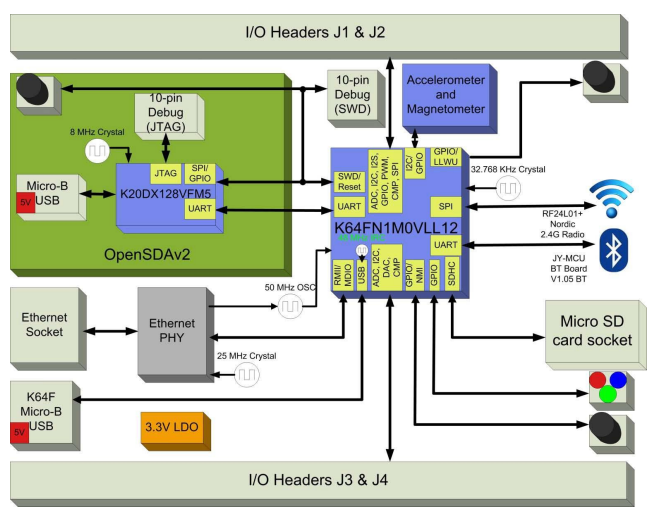
\includegraphics[width=0.9\textwidth]{diagBloquesK64F}
	\caption{Diagrama de bloques placa FRDM K64F.}\label{diagBloquesK64F}
\end{figure}

En el caso de los sistemas embebidos, cada uno de ellos se construye según el propósito específico que se va a realizar con ello, es decir, dependiendo de su objetivo tendrá unas características hardware u otras. Sin embargo, sí que hay algunos componentes mínimos presentes en todas las placas como pueden ser por ejemplo, un microcontrolador (MCU) encargado de controlar las operaciones del SE. \\
Un MCU está compuesto por un procesador, memoria RAM y ROM y puertos de entrada y salida. El MCU se encarga de ejecutar las instrucciones del programa cargado en memoria, en otras palabras, gestiona las entradas y salidas de datos. Además de este componente, necesitaríamos de más periféricos para obtener algunas funcionalidades más específicas, algunos de los periféricos que podríamos utilizar son:

\begin{itemize}
\item Sensores: humedad, temperatura, ultrasonidos, etc.
\item Actuadores: motores, leds, altavoces, etc.
\item Dispositivos de interfaz humana.
\end{itemize}


\subsection{Software}

El software embebido o empotrado reside en memoria de sólo lectura. Con relación al software y hardware utilizados en este proyecto existen 2 posibilidades de cara a cargar el programa en el microcontrolador \cite{embos}:
\begin{itemize}
\item MBED. Este es el modo en el que vienen las placas por defecto. En este modo, al conectar la placa al ordenador aparecerá como un medio extraíble y deberemos arrastrar los ficheros `.bin' en el que estaría el desarrollo de nuestro programa.
\item OpenSDA. (Open Serial and Debug Adapter) o adaptador para depuración serie y comunicación serial en castellano. OpenSDA es la interfaz de bajo costo que ofrece NXP para la depuración y programación de sus microcontroladores. En la Figura \ref{OpenSDA} encontramos su diagrama de bloques.
\end{itemize}

%\imagen{openSDA}{Diagrama de bloques de OpenSDA} \label{OpenSDA}
\begin{figure}[!h]
	\centering
	\includegraphics[width=0.6\textwidth]{openSDA}
	\caption{Diagrama de bloques de OpenSDA.}\label{OpenSDA}
\end{figure}

\clearpage

En el caso de este proyecto es necesario diferenciar algunos conceptos en lo relativo al software:

\begin{description}
\item[SO en tiempo real. \cite{SOTR} \label{ref:SOTiempoReal}] Es un sistema operativo que se utiliza para facilitar la gestión de multitareas en dispositivos con recursos y tiempos limitados \cite{SisTiempoReal}. Además, las tareas deben ser deterministas en el tiempo de ejecución. Para poder comprender adecuadamente la utilidad de un RTOS debemos conocer los siguientes conceptos:
\begin{description}
\item[Tarea.] Las tareas, a las cuales también podemos referirnos como procesos o hilos, se ejecutan de manera independiente, esto quiere decir que tienen su propio espacio de memoria. El aislamiento del espacio de memoria se garantiza mediante protección por hardware (MPU) restringiendo su acceso. Las tareas pueden tener diferentes estados según lo determine el RTOS:
	\begin{description}
		\item[Bloqueado.] La tarea está esperando un evento que puede ser un bloqueo de tipo mutex o semáforo, o una liberación de espacio en memoria .
		\item[Listo.] La tarea está lista para ejecutarse en la CPU, pero se mantiene a la espera porque la CPU ya está siendo utilizada.
		\item[En ejecución.] La tarea se está llevando a cabo.
	\end{description}
Existen distintas técnicas para la programación de estos SO:
	\begin{description}
		\item[Expropiativo.] Se ejecuta la tarea con mayor prioridad. Incluso se puede interrumpir una tarea en curso si hay otra lista con prioridad mayor. Esto tiene una mayor carga en el microcontrolador ya que tiene que gestionar el cambio de tarea.
		\item[No Expropiativo] La ejecución de la tarea es ininterrumpida y solo se detiene su ejecución si se detiene o cede el control voluntariamente.
	\end{description}
\item[Comunicación entre tareas.] Como ha ocurrido en el software realizado es común que algunas variables locales de alguna tarea deban ser utilizadas en otras tareas. Para ello existen dos opciones. La primera y más simple es la utilización de variables globales. La segunda opción es la utilización de colas y buzones que nos modifiquen o lean el valor de esa variable.
\end{description}
\item[Middelware.] Este software se encarga de `comunicar' el sistema operativo con los programas. Es un conjunto de librerías que sirven como rutinas para crear una infraestructura que ofrece servicios a los desarrolladores. Un ejemplo de \extranjerismo{middleware} seria la librería lwIP que se ha utilizado en el software del proyecto.
\item[Drivers.] Los \extranjerismo{drivers} \cite{drivers} o controladores de dispositivos proveen las instrucciones necesarias para que un dispositivo externo, por ejemplo un periférico, pueda ser controlado por el sistema operativo que el sistema embebido utilice. Dos de los \extranjerismo{drivers} más utilizados en este proyecto han sido, enet para configurar el correcto funcionamiento de la conexión en red vía cable ethernet y el \extranjerismo{driver} ADC para poder utilizar los potenciómetros.
\end{description}


\section{Tecnologías de comunicación para SE}\label{sec:Comunicaciones}

Los sistemas empotrados son capaces de comunicarse de varias formas, tanto con periféricos como entre dos o más SE. Algunas tecnologías para comunicarse entre SE serían \extranjerismo{bluetooth}, infrarrojos o wifi, entre otros. De esta manera conseguimos que podamos enviar y recibir información de otros sistemas. \\
Para la comunicación con los periféricos existen otras tecnologías acorde a sus necesidades durante el intercambio de datos. 
En los próximos dos apartados hablaremos sobre este tipo de tecnologías de comunicación y sus utilidades específicas. 

\subsection{Comunicación mediante TCP/IP}

En este apartado vamos a hablar sobre la comunicación mediante TCP/IP. \\
Se explicará cómo se lleva a cabo la comunicación en red vía cable ethernet, que es la que se ha usado en el resultado final del proyecto. Se profundizará en los protocolos que componen el modelo TCP/IP \cite{avastTcpIp} que ha sido utilizado para el establecimiento de conexión en red, envío de paquetes y cierre de la conexión en el software del proyecto. \\


\subsubsection{Modelo TCP/IP}
IBM \cite{IBMTCP} define un protocolo como ``Los protocolos son conjuntos de normas para formatos de mensaje y procedimientos que permiten a las máquinas y los programas de aplicación intercambiar información. Cada máquina implicada en la comunicación debe seguir estas normas para que el sistema principal de recepción pueda interpretar el mensaje.'' \\
Podríamos compararlo con las normas sintácticas que seguimos los humanos para hablar y entendernos los unos a los otros. En este apartado, vamos a centrarnos en el conjunto de protocolos TCP/IP que se dividen en capas o niveles. \\
La figura \ref{disposicionCapas} muestra la disposición de las capas del modelo TCP/IP.

%\imagen{protocolo-TCPIP}{Capas del modelo TCP/IP} \label{disposicionCapas}
\begin{figure}[!h]
	\centering
	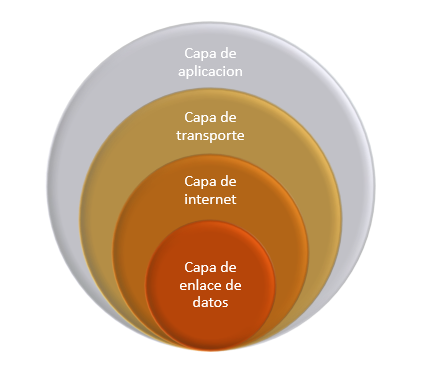
\includegraphics[width=0.9\textwidth]{protocolo-TCPIP}
	\caption{Capas del modelo TCP/IP.}\label{disposicionCapas}
\end{figure}


\begin{description}
\item[Capa de enlace de datos \cite{CapaEnlaceDatos}] 
Esta capa se encarga del intercambio de datos entre un \extranjerismo{host} y la red a la que se está conectado. Su objetivo es establecer una correcta comunicación entre las capas superiores (Red, Transporte y Aplicación) y el medio físico de transporte de datos. Esta comunicación debe ser segura entre los dos nodos, implementa un sistema de notificación de errores de la topología de la red y el control en la transmisión de las tramas. 
Esta capa se encarga de la transmisión y direccionamiento de datos sin errores y con seguridad entre nodos que pertenezcan a la misma red (comunicación punto a punto), a través del medio físico . Por otro lado, la capa de Red que es la encargada de la transmisión y direccionamiento de datos entre \extranjerismo{host} que se encuentran en redes diferentes. Ambas capas trabajan conjuntamente, puesto que la capa de Enlace de datos proporciona sus servicios a la capa de Red, ofreciendo una transmisión de datos confiable a través de un enlace físico.
Como resumen de sus principales funciones tenemos:
\begin{itemize}
\item Proporciona los servicios y medios necesarios para establecer una comunicación confiable y eficiente entre dos \extranjerismo{host}. Para ello agrega una secuencia de bits al inicio y final de los paquetes bajo un formato predefinido formando tramas.
\item Añade bits de paridad para ejercer un control de errores en el envío de las tramas. Estos bits son CRC (Códigos Cíclicos Redundantes)
\item Envía los paquetes de nodo a nodo.
\item Regula la congestión de la red.
\item Gestiona la velocidad del tráfico de datos.
\end{itemize}

\item[Capa de Internet]
La capa de Internet \cite{lopezQuesadaRED} (también denominada capa de red) controla el movimiento de los paquetes alrededor de la red. Se encarga del direccionamiento de los dispositivos y del empaquetado y manipulación de los datos para su correcto envío, entre \extranjerismo{host} que pueden estar ubicados en redes geográficamente distintas. Su misión es conseguir que los datos lleguen a su destino aunque no tengan conexión directa. Para conseguir su objetivo, ofrece servicios al nivel superior (capa de transporte) y se apoya en la capa de enlace de datos para encaminar los paquetes, mantener un control de la congestión de la red y el control de errores. 
Esta capa utiliza las versiones IPV4 e IPV6 para el encaminamiento, control y notificación de errores, existe además, IGMP (Internet Group Management Protocol) y MLD (Multicast Listener Discovery) que se usan para establecer grupos de difusión múltiple.

El protocolo IP determina el destinatario del mensaje mediante 3 elementos:
\begin{itemize}
\item Dirección IP: Dirección del equipo.
\item Máscara de subred: una máscara de subred le permite al protocolo IP establecer la parte de la dirección IP que se relaciona con la red.
\item Gateway(Puerta de enlace): le permite al protocolo de Internet saber a qué equipo enviar un datagrama, si el equipo de destino no se encuentra en la red de área local.
\end{itemize}

\item[Capa de Transporte]
La capa de transporte \cite{capaTransporte} se encarga de la segmentación de datos y ensamblaje de las partes dentro de los canales de comunicación. Esta capa se asegura de conseguir que la conexión de datos sea fiable entre dos dispositivos. Para ello, envía los datos en paquetes y se asegura de que el otro equipo indique que ha recibido los paquetes correctamente. En otras palabras, se encarga de facilitar la comunicación lógica entre dispositivos. Esta comunicación puede utilizar dos protocolos:
	\begin{description}
	\item[TCP] es un protocolo orientado a la conexión, proporciona un conjunto completo de servicios para aquellas aplicaciones que lo necesiten y su uso se considera fiable. Con el uso de puertos consigue que varias aplicaciones puedan usar una misma dirección IP. El protocolo establece una conexión virtual entre dos dispositivos capaz de enviar información de manera bidireccional. 
	\item[UDP] A diferencia de TCP, UDP no utiliza ningún mecanismo de establecimiento de la conexión, no dispone de mecanismo que aseguren, la transferencia fiable de los segmentos, por lo tanto, determinados segmentos pueden llegar a perderse. Su uso se justifica en aquellos escenarios donde la velocidad de la transmisión prima por encima de todo, aunque se incurra ocasionalmente en la pérdida de información.
	\end{description}

\item[Capa de aplicación]
Esta capa nos ofrece la posibilidad de acceder a otras capas para usar sus servicios \cite{protocolosAplicacion}. Además a esta capa, pertenecen protocolos como:
\begin{itemize}
\item Sistema de nombres de dominios (DNS): este protocolo relaciona nombres de Internet en direcciones IP.
\item Telnet: Proporciona acceso remoto a servidores y dispositivos de red.
\item Protocolo simple de transferencia de correo (SMTP): Se usa para enviar mensajes y archivos adjuntos de correo electrónico.
\item Protocolo de configuración dinámica de host (DHCP): Este protocolo asigna una dirección IP y direcciones de máscara de subred, de gateway predeterminado y de servidor DNS a un host.
\item Protocolo de transferencia de hipertexto (HTTP): Se encarga de transferir los archivos que conforman las páginas Web de la World Wide Web.
\item Protocolo de oficina de correos (POP): Es utilizado por los clientes de correo electrónico para recuperar el correo electrónico de un servidor remoto.
\item Protocolo de acceso a mensajes de Internet (IMAP): Se utiliza para recuperar correo electrónico.
\end{itemize}
Los protocolos nombrados, son usados tanto por los dispositivos de origen como de destino durante la comunicación.
\end{description}


\section{Comunicaciones para los periféricos}
Como ya mencionamos anteriormente, la mayor funcionalidad que podemos dar a estas placas viene con la condición de poder comunicarnos entre ellas y con otros periféricos. Veamos algunos tipos de conexión, además de vía ethernet o wifi, que hemos utilizado en este trabajo.

\subsection{UART}
UART, 'Universal Asynchronous Receiver-Transmitter' o en castellano Receptor-transmisor asíncrono universal. Su funcionamiento es sencillo. Utiliza solamente dos hilos para transmitir los datos. Las conexiones son cruzadas entre los dos dispositivos, es decir el pin de transmisión (TX) del dispositivo que emite el mensaje, estará conectado al pin receptor (RX) del dispositivo que recibe la comunicación y viceversa. Esta comunicación es asíncrona, por lo que no utiliza relojes para el envío y recepción de mensajes. 
Para que ambos dispositivos sepan cuando tienen que empezar y dejar leer bits se añaden a cada envío bits de inicio y parada. Es importante que ambos equipos tengan la misma tasa de Baudios configurada para que los bits se lean adecuadamente, de no ser así, la comunicación fallaría ya que un dispositivo enviaría bits a una velocidad diferente de la que se leen, ocasionando lecturas erróneas. La velocidad predeterminada suele ser de 9600 baudios. En la Figura \ref{figTramaUart} podemos ver los bits que forman una trama UART \cite{queEsUART}:

%\imagen{tramaUART}{Trama UART} \label{figTramaUart}
\begin{figure}[!h]
	\centering
	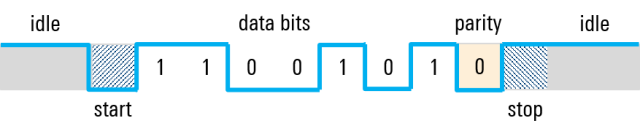
\includegraphics[width=0.9\textwidth]{tramaUART}
	\caption{Trama UART.}\label{figTramaUart}
\end{figure}

Como podemos observar los bits que forman la trama son:
\begin{itemize}
\item Bits de inicio y parada. Puesto que UART es asíncrono, son necesarios para que el receptor sepa desde dónde tiene que empezar a leer y cuando parar.
\item Bits de datos. Son la carga útil, puede haber de 5 a 9 bits por trama. 
\item Bit de paridad. Este bit se utiliza para la detección de errores en las tramas. Existen dos tipos de paridad, paridad par o impar. 
\end{itemize}

Por otro lado tenemos la comunicación USART ‘Universal Synchronous and Asynchronous Receiver-Transmitter’ que puede realizar procesos de comunicación con relojes. En la Tabla \ref{tabla:DiferenciasUART} podremos ver sus diferencias \cite{DifUartUsart} principales:

\tablaSmallSinColores{Diferencias USART y UART}{l c c}{DiferenciasUART}
{\multicolumn{1}{c}{Características} & USART & UART\\}
{
Modo & Semidúplex & Dúplex\\
Velocidad & USART es mayor & UART es menor.\\
Funcionamiento & Señales de datos y de reloj & Señales de datos\\
Datos & Bloques	& Bytes \\
Complejidad & Más complejo & Más simple de utilizar\\ 
}


El principal motivo de hacerlo con UART en vez de con USART, es su sencillez. Además los comandos de los motores se envían en bytes y no en bloques, por lo que es más directo hacerlo con UART.

\subsubsection{I2C}
El protocolo I2C, 'Inter-Integrated Circuit' usa dos líneas para comunicarse con otros dispositivos, además de las líneas de tierra y voltaje. Por un lado tenemos SCL (línea de reloj en serie) y por otro lado tenemos SDA (línea de datos), esta última es la encargada de transmitir la información. Mediante estas dos líneas el protocolo I2C es capaz de enviar datos de forma segura. Veamos algunos de los bits importantes que, tanto el maestro y esclavo \cite{hetProI2c} pueden utilizar para formar y leer las tramas:
\begin{itemize}

\item Inicio ó Start – S
\item Parada – P
\item Confirmación – ACK
\item NoConfirmación – NACK
\item Lectura-/Escritura – L/W
\item 7 bits para la dirección del dispositivo esclavo/maestro
\item 8 bits de dirección ( para algunos sensores pueden ser 16 bits)
\item 8 bits de datos
\end{itemize}
Existen distintos modos de comunicación, dependiendo de esos modos se utilizarán distinto orden y número de bits para formar las tramas. Los modos principales de comunicación son:
\begin{itemize}
\item Maestro-Transmisor y Esclavo-Receptor. Este modo se usa cuando se desea configurar un registro del esclavo I2C.
\item Maestro-Receptor y Esclavo-Transmisor. Se usa cuando queremos leer información del sensor I2C.
\end{itemize}

Este tipo de comunicación suele estar destinada al intercambio de datos con módulos o sensores y se usa en arquitecturas maestro-esclavo. Varios esclavos pueden estar conectados a un maestro al mismo tiempo pero, como es lógico, cuantos más esclavos estén conectados al maestro mayor latencia habrá en el envío y recepción de datos. Esto se debe a que solo se puede usar el bus I2C para comunicar un esclavo al mismo tiempo. También hay que tener en cuenta que dos maestros no pueden utilizar el mismo puerto. Veamos las características del maestro y el esclavo:
\begin{itemize}
\item Maestro: Dispositivo que proporciona un reloj para la comunicación. Sus funciones principales son:
\begin{enumerate}
\item Iniciar la comunicación – S
\item Enviar 7 bits de dirección – ADDR
\item Generar 1 bit de Lectura o Escritura – R/W
\item Enviar 8 bits de dirección de memoria
\item Transmitir 8 bits de datos –
\item Confirmar la recepción de datos – ACK – ACKnowledged
\item Generar confirmación de No-recepción, NACK – No-ACKnowledged
\item Finalizar la comunicación
\end{enumerate}
\item Esclavo: Dispositivo que utiliza el reloj del maestro. Sus funciones principales son:
\begin{enumerate}
\item Enviar información en paquetes de 8 bits.
\item Enviar confirmaciones de recepción, llamadas ACK.
\end{enumerate}
\end{itemize}
En nuestro caso, utilizamos este tipo de comunicación para el uso de la pantalla LCD.



\section{Periféricos}\label{sec:perifericos}
En esta parte de la memoria, vamos a ver las especificaciones de los periféricos utilizados en este proyecto

\subsection{Potenciómetro y sensor de temperatura} \label{potenySensorTemp}

El potenciómetro \cite{Potenciometro} es un elemento hardware que busca determinar un potencial eléctrico en una conexión. Generalmente, se consigue mediante la comparación de la potencia de entrada y la de salida. Esta diferencia de potencial es lo que se conoce como voltaje.
Su funcionamiento es sencillo, cuenta con tres resistencias, dos en cada uno de los extremos y una tercera resistencia con la cual podemos interactuar, permitiéndonos aumentar o disminuir su valor.

Un sensor de temperatura \cite{TempSens} es un dispositivo que transforma los cambios de temperatura (magnitud física) en señales eléctricas(voltaje). Por lo general, está  formado por un sensor encapsulado en una cubierta protectora. Entre el sensor y la cápsula encontramos un material que es  conductor térmico y que permite traspasar rápidamente estos cambios de temperatura. Existen tres tipo de sensores de temperatura descritos perfectamente en \cite{TempSensTipos}:

\begin{itemize}
\item Termopares. Funcionan mediante un principio de generación de una corriente entre dos metales diferentes unidos que tienen diferente comportamiento eléctrico en función de la temperatura. La señal generada se procesa y da lugar a una medición de temperatura. Son equipos sencillos, baratos y con una precisión suficiente para su uso en edificación. Sin embargo, tienen una respuesta lenta.
\item Termorresistencias. Están constituidas por resistencias cuya conductividad varía en función de la temperatura, lo cual genera una señal que, una vez procesada, permite obtener la medición de temperatura. Su velocidad de respuesta depende de la masa de la resistencia.
\item Sensores electrónicos. Funcionan mediante dispositivos electrónicos que generan una corriente o señal en función de la temperatura. Son equipos con una respuesta mucho más rápida, pero más caros.
\end{itemize}


